

\section{Understandability Study (RQ2)}
\label{sec:understandability}
The overall idea of this study  is to present  programmers with one of several representations of semantically equivalent regexes and ask comprehension questions. By comparing the understandability of semantically equivalent regexes that have different representations, we aim to understand which representation(s)  are more desirable and which are more smelly. 
This study was  implemented on Amazon's Mechanical Turk with 180 participants.  Each regex was evaluated by 30 participants. 
The regexes used were designed to belong to various representations in Figure~\ref{fig:refactoringTree}. 



\begin{figure}[tb]
\centering
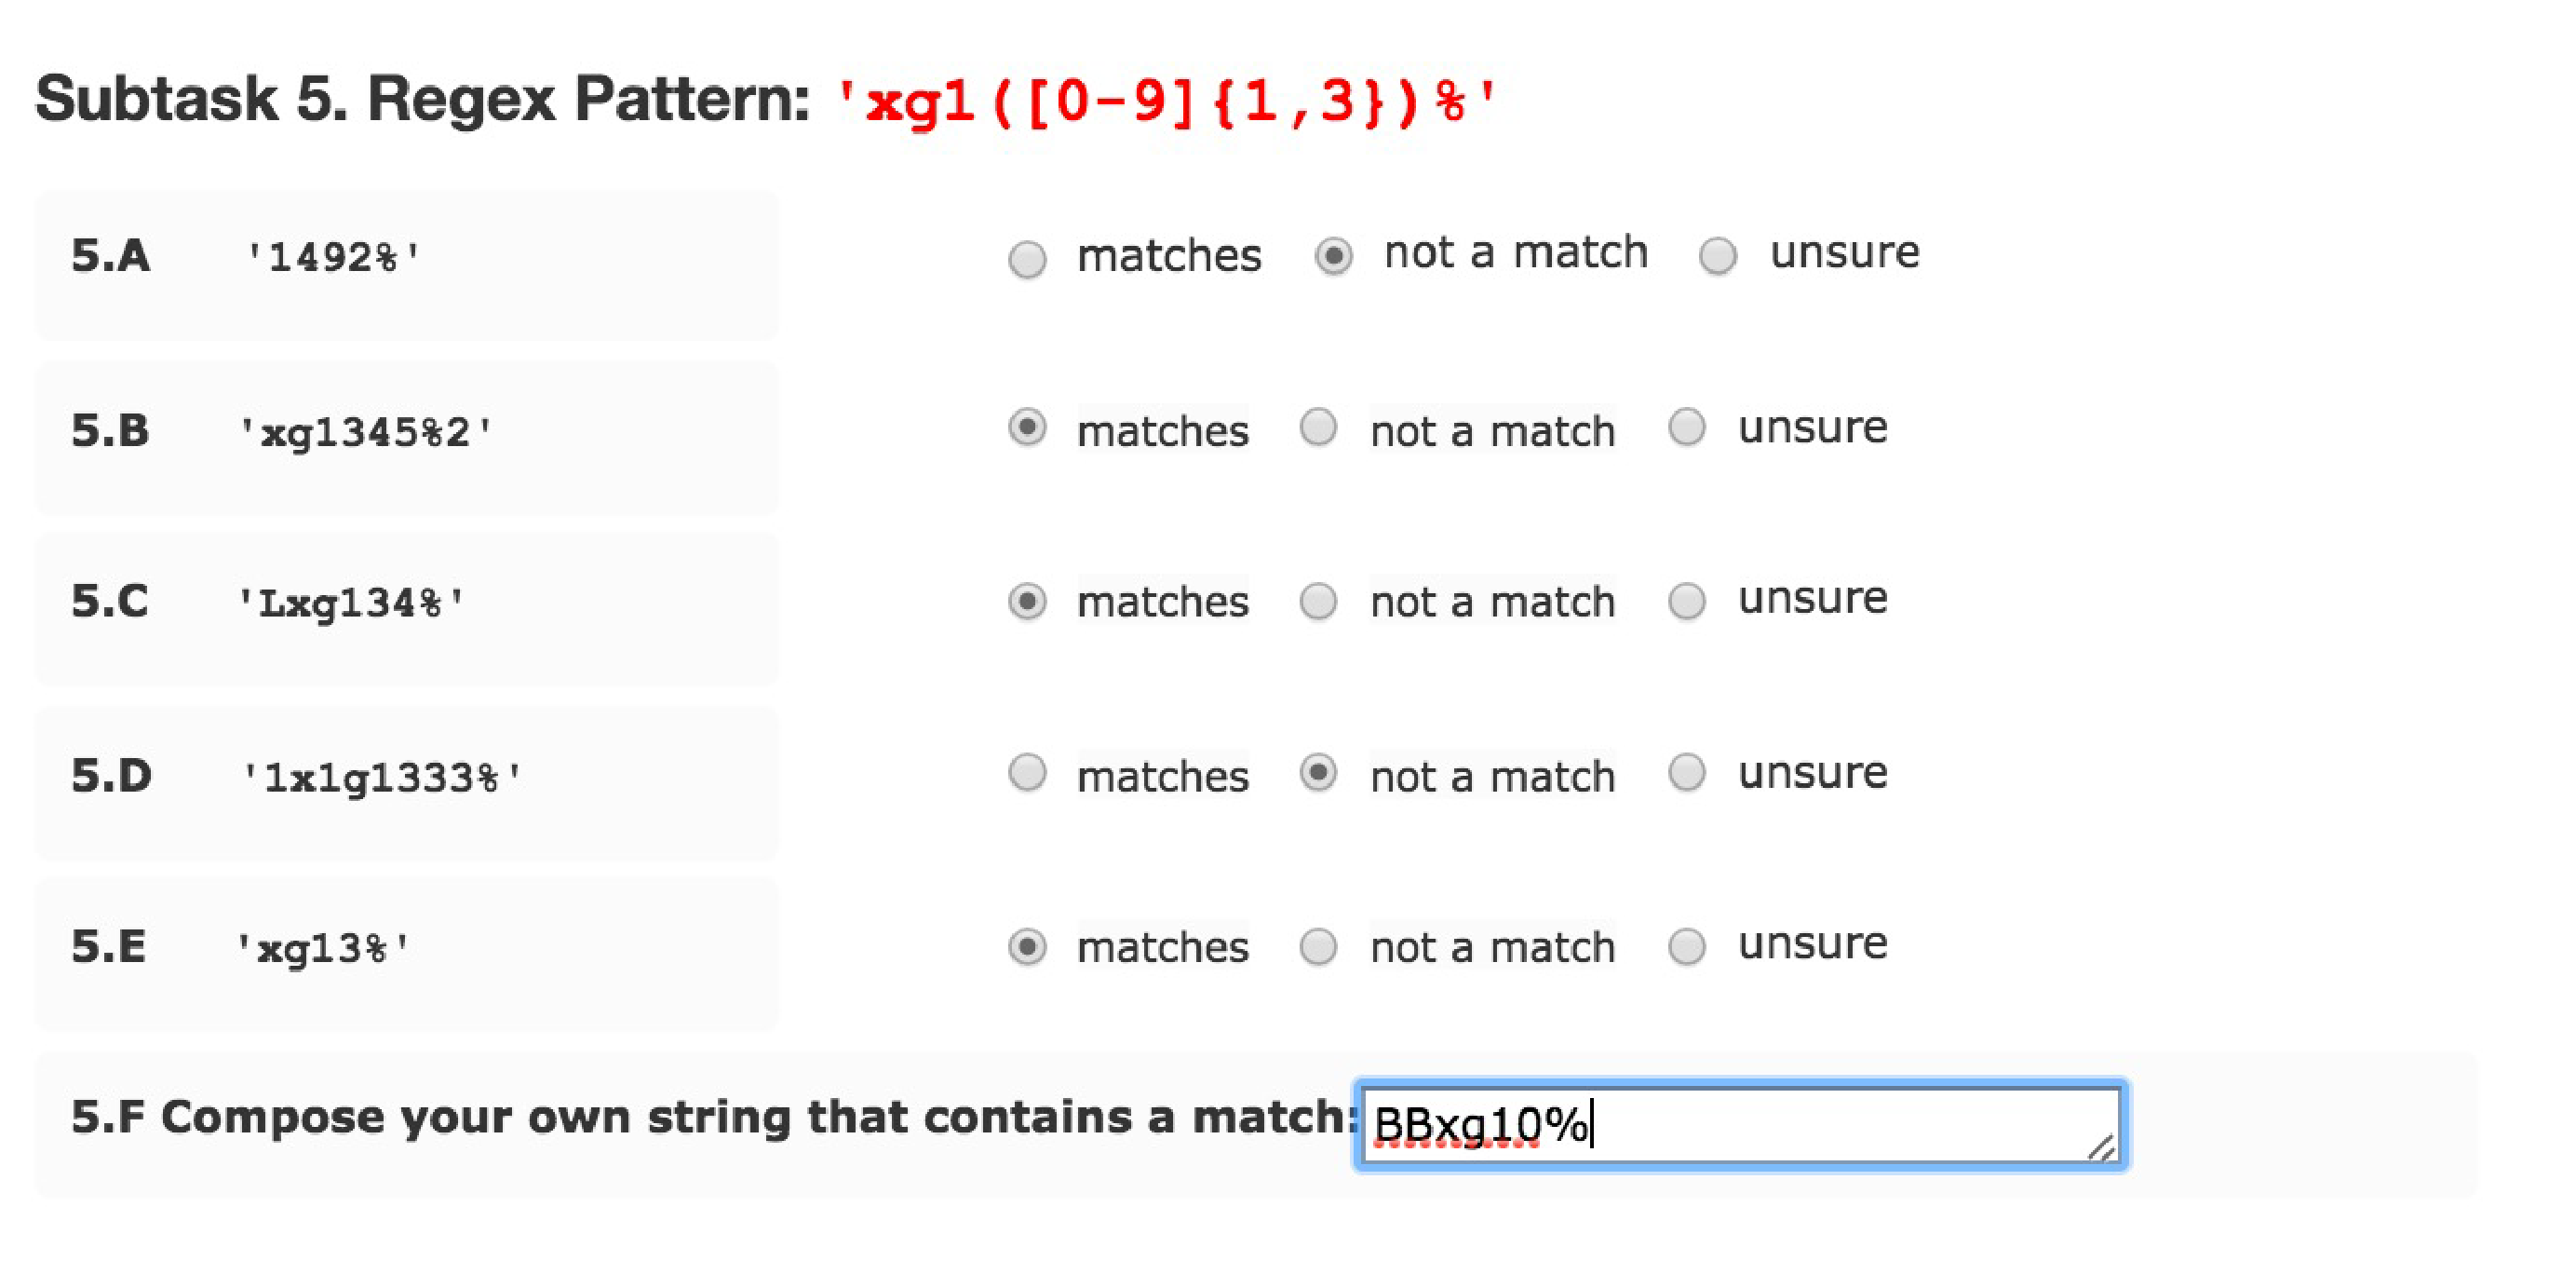
\includegraphics[width=\columnwidth]{illustrations/exampleQuestion}
\vspace{-12pt}
\caption{Example of one HIT Question}
\vspace{-6pt}
\label{fig:exampleQuestion}
\end{figure}

%In Mechanical Turk, we designed a 180 tasks composed of 10 matching subtasks, so that each of the 60 CRs had 30 separate observations (each an average of 5 \emph{example string} problems).  These 1800 observations are what the analysis will focus on. The ordering of the regexes in each HIT was random to control for learning effects.


\begin{table}
\caption{Matching metric example \label{matchingmetric}}
\begin{center}
\begin{small}
\begin{tabular} {cl | c c c c c}
\textbf{String} & \verb!`RR*'! & \textbf{Oracle} & \textbf{P1} & \textbf{P2} & \textbf{P3}& \textbf{P4}\\ \hline
1 & ``ARROW"    & \checkmark    & \checkmark    & \checkmark    & \checkmark    & \checkmark \\
2 & ``qRs"      & \checkmark    & \checkmark    & \xmark        & \xmark        & ?\\
3 & ``R0R"      & \checkmark    & \checkmark    & \checkmark    & ?             & -\\
4 & ``qrs"      & \xmark        & \checkmark    & \xmark        & \checkmark    & -\\
5 & ``98"       & \xmark        & \xmark        & \xmark        & \xmark        & -\\
\hline
  & Score       & 1.00          & 0.80          & 0.80          & 0.50          & 1.00\\
\\
\multicolumn{7}{l}{\checkmark = match, \xmark = not a match, ? = unsure, -- = left blank}\\
\end{tabular}
\end{small}
\end{center}
\end{table}





\subsection{Metrics}
\label{sec:understadningmetric}
 We measure the understandability of regexes using two complementary metrics, \emph{matching} and \emph{compostition}.


\textbf{Matching:}
 Given a regex and a set of strings, a participant determines which strings will be matched by the regex. There are four possible responses for each string, \emph{matches}, \emph{not a match}, \emph{unsure}, or blank. An example from our study is shown in Figure~\ref{fig:exampleQuestion}. 
 
 The percentage of correct responses, disregarding blanks and unsure responses, is the matching score. 
 For example, consider regex \verb!`RR*'! and five strings, which comes from our study, shown in Table~\ref{matchingmetric}, and the responses from four participants in the \emph{P1}, \emph{P2}, \emph{P3} and \emph{P4} columns. 
 The oracle has the first three strings matching since they each contain at least one \verb!R! character. \emph{P1} answers correctly for the first three strings but incorrectly thinks the fourth string matches, so the matching score is $4/5 = 0.80$. \emph{P2} incorrectly thinks that the second string is not a match, so they also score $4/5 = 0.80$.  \emph{P3} marks `unsure' for the third string and so the total number of attempted matching questions is 4 instead of 5. \emph{P3} is incorrect about the second and fourth string, so they score $2/4 = 0.50$.  For \emph{P4}, we only have data for the first and second strings, since the other three are blank.  \emph{P4} marks `unsure' for the second matching question so only one matching question has been attempted, and it was answered correctly so the matching score is $1/1 = 1.00$.
 
Blanks were incorporated into the metric because questions were occasionally left blank in the study. Unsure responses were provided as an option so not to bias the  results when participants were honestly unsure of the answer. These situations did not occur very frequently. Only \todoNow{X\%} of the responses were left blank and only \todoNow{y\%} of the responses were marked as unsure.   


\textbf{Composition:}
Given a regex, a participant composes a string they think it matches. If the participant is accurate and the string indeed is matched by the regex, then a composition score of 1 is assigned, otherwise 0.  For example, given the regex \verb!`(q4fab|ab)'! from our study, the string, ``xyzq4fab" matches  and would get a score of 1, and the string, ``acb" does not match and would get a score of 0.

To determine a match, each regex was compiled using the \emph{java.util.regex} library. A \emph{java.util.regex.Matcher} \verb!m! object was created for each composed string using the compiled pattern.  If \verb!m.find()! returned true, then that composed string was given a score of 1, otherwise it was given a score of 0.



\subsection{Design}
%\todoNow{needs to be updated with respect to no C1,T1 nodes}
This study was implemented on the Amazon's Mechanical Turk (MTurk),  a crowdsourcing platform in which requestors can create human intelligence tasks (HITs) for completion by workers. Each HIT is designed to be completed in a fixed amount of time and workers are compensated with money if their work is satisfactory. Requesters can screen workers by requiring each to complete a qualification test prior to completing any HITs. 

\subsubsection{Worker Qualification}
Workers were pre-qualified by answering questions regarding some basics of regex knowledge. These questions were multiple-choice and asked the worker to describe what the following regexes mean: \verb!a+!, \verb!`(r|z)'!, \verb!`\d'!, \verb!`q*'!, and \verb![p-s]'!. To pass the qualification, workers had to answer four of the five questions correctly.

\subsubsection{Tasks}
Using the regexes in the corpus as a guide, we created 60 regex patterns that were grouped into 26 semantically equivalence groups, where 18 groups had two equivalent regexes each and eight groups had three equivalent regexes each. For example, one of the groups of size two had regexes, \verb!([0-9]+)\.([0-9]+)'! belonging to representation C1 and \verb!(\d+)\.(\d+)'! belonging to representation C4. One of the groups of size thee contained \verb!((q4f)?ab)'! belonging to D2, \verb!(q4fab|ab)'! belonging to D3, and \verb!((q4f){0,1}ab)'! belonging to D1. 
For each of the 26 groups of regexes, we created five strings, where at least two matched and at least two did not match. The fifth string was randomly selected to match or not match. These strings were used to compute the matching metric. 
%These were used for computing the composition metric.

Once all the regexes and matching strings were collected, we created tasks for the MTurk participants as follows: randomly select a regex from ten of the 26 groups. Randomize the order of the regexes, as well as the order of the matching strings for each regex. After adding a question asking the participant to compose a string that the regex matches, this creates one task on MTurk.   This process was completed until each of the 60 regexes appeared in 30 HITs, resulting in a total of 180 total, unique HITs.
An example of a single regex, the five matching strings and the space for composing a string is shown in Figure~\ref{fig:exampleQuestion}.


\subsubsection{Implementation}
Workers were paid \$3.00 for successfully completing a HIT, and were only allowed to complete  one HIT.  The average completion time for accepted HITs was 682 seconds (11 mins, 22 secs).  
%A total of 241 HITs were submitted - of those 55 were rejected.
%, and 6 duplicates were ignored, always using the first accepted submission so as to obtain a value for each of the 180 distinct tasks.
A total of 55 HITs were rejected, and  of those, 48 were rushed through by one person leaving many answers blank, 4 other HITs were also rejected because a worker had submitted more than one HIT, one was rejected for not answering composition sections, and one was rejected because it was missing data for 3 questions.  Rejected HITs were returned to MTurk to be completed by others.


%
%
%
%\begin{figure}[tp]
%\begin{small}
%\fbox{\parbox{\columnwidth}{
%\begin{enumerate}
%\item
%\begin{tabular} {lrr}
%\textbf{What is your gender?} & \textbf{n} & \textbf{\%}\\ \hline
%Male & 149 & 83\%\\
%Female & 27& 15\%\\
%Prefer not to say & 4& 2\%
%\end{tabular}
%\item \textbf{What is your age?} \\
%$\mu = 31$, $\sigma = 9.3$
%
%\item
%
%\begin{tabular} {l |rr}
%\textbf{Education Level?} & \textbf{n} & \textbf{\%}\\ \hline
%High School & 5 & 3\%\\
%Some college, no degree & 46 & 26\%\\
% Associates degree & 14 & 8\%\\
%Bachelors degree & 78 & 43\%\\
%Graduate degree & 37 & 21\%\\
%\end{tabular}
%\item
%\begin{tabular} {lrr}
%\textbf{Familiarity with regexes?} & \textbf{n} & \textbf{\%}\\ \hline
%Not familiar at all & 5 & 3\%\\
%Somewhat not familiar & 16 & 9\%\\
%Not sure & 2 & 1\%\\
%Somewhat familiar & 121 & 67\%\\
%Very familiar & 36 & 20\%\\
%\end{tabular}
%\item \textbf{How many regexes do you compose each year?} \\
%$\mu = 67$, $\sigma = 173$
%\item \textbf{How many regexes (not written by you) do you read each year?} \\
%$\mu = 116$, $\sigma = 275$
%%\item In what contexts do you use regexes? \\
%\end{enumerate}
%}}
%\caption{Participant Profiles, $n=180$ \todoLast{can remove this for space} \label{participantprofile}}
%\end{small}
%\end{figure}
%


\subsection{Participants}

In total, there were 180 participants in the study.
A majority were male (83\%) with an average age of 31. Most had
at least an Associates degree (72\%) and most were at least somewhat familiar with regexes prior to the study (87\%). On average,
participants compose 67 regexes per year with a range of 0 to 1000. Fittingly, participants read more regexes than they write with an average of 116 and a range from 0 to 2000. 
%Figure~\ref{participantprofile} summarizes the self-reported participant characteristics from the qualification survey.

\begin{table*}\begin{small}\begin{center}\caption{Averaged Info About Edges}\label{table:testedEdgesTable}\begin{tabular}
{llccccccc}
index & edge & nExp & acc1 & acc2 & cmp1 & cmp2 & Pacc & Pcmp \\
\toprule[0.16em]
E1 & C1 -- C2 & 2 & 0.94 & 0.90 & 28.0 & 27.0 & 0.268800 & 0.802400\\
E2 & C1 -- C2, T2  -- T1 & 2 & 0.84 & 0.86 & 19.5 & 27.5 & 0.751200 & 0.031185\\
E3 & C1 -- C2,T4->T1 & 2 & 0.81 & 0.86 & 15.5 & 27.5 & 0.609700 & 0.022661\\
E4 & C1->C4 & 5 & 0.76 & 0.76 & 24.2 & 23.8 & 0.555860 & 0.500942\\
E5 & C1->C5 & 5 & 0.90 & 0.88 & 27.0 & 27.2 & 0.472560 & 0.551300\\
E6 & C2->C4 & 1 & 0.83 & 0.92 & 18.0 & 20.0 & 0.075020 & 0.788800\\
E7 & C2->C5 & 4 & 0.85 & 0.86 & 26.5 & 28.5 & 0.282075 & 0.598075\\
E8 & C2->C5,T4->T1 & 2 & 0.60 & 0.82 & 11.0 & 29.0 & 0.048688 & 0.000015\\
E9 & D1->D2 & 2 & 0.84 & 0.78 & 28.0 & 26.5 & 0.306450 & 0.598350\\
E10 & D1->D3 & 2 & 0.84 & 0.87 & 28.0 & 29.0 & 0.526250 & 0.802400\\
E11 & D2->D3 & 2 & 0.78 & 0.87 & 26.5 & 29.0 & 0.155290 & 0.598350\\
E12 & L2->L3 & 3 & 0.86 & 0.91 & 27.3 & 29.3 & 0.230233 & 0.751533\\
E13 & S1->S2 & 3 & 0.86 & 0.85 & 27.0 & 26.3 & 0.420767 & 1.000000\\
E14 & T1->T3 & 3 & 0.88 & 0.86 & 21.7 & 22.7 & 0.177233 & 0.697267\\
E15 & T1->T4 & 2 & 0.80 & 0.60 & 26.0 & 11.0 & 0.049250 & 0.002759\\
E16 & T2->T4 & 2 & 0.84 & 0.81 & 19.5 & 15.5 & 0.519000 & 0.535040\\
\bottomrule[0.13em]\end{tabular}\end{center}\end{small}\end{table*}



\subsection{Analysis}
For each of the 180 HITs, we computed a matching and composition score for each of the 10 regexes, using the metrics described in Section~\ref{sec:understadningmetric}. This allowed us to compute 30 values for each metric and for each of the 60 regexes. Next, we computed average scores for matching and composition per regex. 

Each regex was a member of one of 26 groupings of equivalent regexes. These groupings allow pairwise comparisons of the metrics values to determine which representation of the regex was most understandable. Among all the groups, we performed 42 pairwise comparisons of the matching and composition scores  (i.e., one comparison for each group of size two and three comparisons within each group of size three). 
For example, one group of size two had regexes, \verb!RR*! and \verb!R+!, which are equivalent and represent a transformation between L2 and L3. The former had an average matching of \todoNow{X} and the latter had an average matching of \todoNow{Y}. The average composition score for the former was \todoNow{Z} and \todoNow{W} for the latter. Thus, the community found \todoNow{state the regex} from representation \todoNow{L?} more understandable. There were two other pairwise comparisons performed between the L2 and L3 group, using regexes pair \verb!zaa*! and \verb!za+'!, and regexes pair \verb!\..*! and \verb!\.+'!. Considering all three of these regex pairs, the overall matching average for the regexes belonging to L2 was 0.86 and 0.91 for L3. The overall composition score for L2 was 0.91 and 0.98 for L3. Thus, the community found L3 to be more understandable, from the perspective of both understandability metrics, than L2. 
This information is presented in summary in Table~\ref{table:testedEdgesTable}, with this specific example appearing in the E3 row. The \emph{Index} column enumerates all the pairwise comparisons evaluated in this experiment, \emph{Representations} lists the two representations, \emph{Pairs} shows how many comparisons were performed, \emph{Match1} gives the overall matching score for the first representation listed, \emph{Match2} gives the overall matching score for the second representation listed, and $H_0: \mu_{match1} = \mu_{match2}$ uses the Mann-Whitney test of means to compare the matching scores, and presents the p-values. The last three columns list the average composition scores for the representations and the p-value, also using the Mann-Whitney test of means. 

%60 strings
%42 comparisons
%18@2, 8@3
%
%M6R1 ? group 3, 3 comparisons
%- 1 comparisons
%- 0 strings
%
%M3R0 ? group 3, 3 comparisons
%- 1 comparisons
%- 0 strings
%
%M3R1 ? group 3, 3 comparisons
%- 2 comparisons
%- 1 string
%
%M3R0 ? group 3, 3 comparisons
%- 2 comparisons
%- 1 string
%
%58 strings
%36 comparisons 


Although we had 42 pairwise comparisons,  we had to drop six comparisons  due to a design flaw since the regex examples performed transformations from multiple equivalence classes. For example, regex \verb!([\072\073])! is in C2 and T4, and was grouped with regex \verb!(:|;)! in C5, T1, so it was not clear if any differences in understandability were due to the transformation between C2 and C5, or T4 and T1. However, the third member of the group, \verb!([:;])!, could be compared with both, since it is a member of T1 and C2, so comparing it to \verb!([\072\073])! evaluates the transformation between T1 and T4, and comparing to \verb!(:|;)! evaluates the transformation between C2 and C5. The end result is 36 pairwise comparisons across 14 edges from Figure~\ref{fig:refactoringTree}. 


%For each of the 60 regexes, an average matching score was computed using the metrics in Table~\ref{matchingmetric}. The average composition metric was measured using the process described in Section~\ref{sec:metric}. This addresses \emph{RQ2} and \emph{RQ3}.

%\todoNow{How to deal with unsure responses? How many were there? Carl's analysis goes here.}



\subsection{Results}
Table~\ref{table:testedEdgesTable} presents the results of the understandability analysis. A horizontal line separates the first three edges from the bottom 11. In E1 through E3, there is a statistically significant difference between the representations for at least one of the metrics considering $\alpha = 0.05$.  These represent the strongest evidence for suggesting the directions of refactoring based on the understandability metrics we defined. Specifically, $\overrightarrow{T4 T1}$, $\overrightarrow{D2 D3}$, and $\overrightarrow{L2 L3}$ 
%T4~$\rightarrow$~T1, D2~$\rightarrow$~D3, and L2~$\rightarrow$~L3 
are likely to improve understandability. 

We note here that participants were able to select \emph{unsure} when they were not sure if a string would be matched by a regex (Figure~\ref{fig:exampleQuestion}). From a comprehension perspective, this indicates some level of confusion and we can use that to further corroborate the understandability analysis. 

\todoNow{incorporate unsure analysis here}

